%=========================================================================
% (c) Michal Bidlo, Bohuslav Křena, 2008

\chapter{Introduction}

The main goal of the project is to design and develop a mechanism for analyzing and notifying users about interesting changes in new uploaded submissions. The mechanism must support a few types of notifications and has possibility to extend types. The changes must also have interface for presentation results. Interested people would be able to set notifications for interesting results of the analyzes.

It is important and useful because the biggest part of the test results are not interesting and has useless information, like the same testing results. Thus, the main goal of the analyzing is to find the interesting results and show them to user.\\Analyzing of submissions is very important because a lot of results are useless, in most cases they are the same data, so it doesn't give any important information. Analyzing helps to save developer's time, it finds useful information and notifies developers or other interested people about that and thus anyone at any time can easily find needed information, or to see statistics of project.\\Firstly, I must learn inner architecture of ResultCloud. How it works. This help me to use better all the opportunities in design and programming that mechanism.

\chapter{Introduction in ResultCloud}

This chapter is describe how ResultCloud work and all important moments for this bachelor's work, like what is submissions and how import of new test cases work.

\section{What is ResultCloud}

ResultCloud is a system for management of long-term testing results. This means that ResultCloud collect testing results of some project and compare it, so developer can easily find the difference between them. Currently, there don't exist new, modern instruments for the collect and the presentate testing results in readable form. As written by Fillip Matys: “Tools which solve that problem [3], are too old and fall behind all modern applications. One of the biggest problem of that tools is no opportunity to expand and with growing market of different mobile devices with internet connection not able to present data in responsive form.” So all instruments that we have now is too old, and doesn't extendable. But in ResultCloud parsing and management doing by modules. Each module is written for one type of testing results. For example module “DejaGnu summary v1.0” can parse and show only SystemTap results. 

\begin{wrapfigure}{r}{0.5\textwidth}
  \centering
    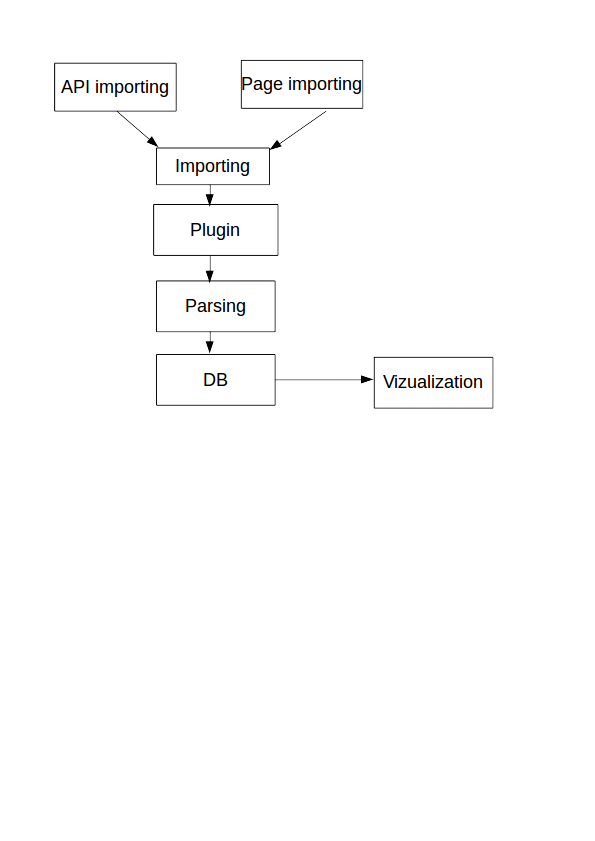
\includegraphics[trim=0 13.41cm 0 0,scale=0.5]{fig/result-cloud.png}
  \caption{ResultCloud architecture}
  \label{fig:result_cloud}
\end{wrapfigure}

ResultCloud is a complex system. ResultCloud consist of two parts frontend and backend. Frontend is a part on the client side, compited with using of AngularJS. Angular in asynchronous format connecting with backend part. Backend also dividing on the smaller part. On the top of hierarchy are Controllers. This hierarchy can be seen in image\ref{fig:result_cloud}. Angular connect directly with controllers. Controllers has only one mission, to get request and parsed data and give it to Services. Services are very important part, they get data and use different database entities, other services, plugins for returning result to the controller, which return it to client. 

For connecting with database there is exist a Driver that connected to database, and use data access object (DAO). DAO consists all basic methods for working with database. Every entity must have DAO, which inherit base DAO, and then system will work with entity through entity's DAO. Results of SELECT query converting to TSE (Test-Suite-Entity) object. TSE object helps to work easier with entities.

Data organization in ResultCloud is represent in Plugins. Plugin is a system for parse and save test's results in specific format. In the past plugins has all demanded for self-installation, parsing and vizualization data, now vizualization is shared. 
Each plugin has own implementation of Parser to parse input data, it is saved in a Project, Submission, etc. Hierarchy of shared entities is following: Projects  contains Submissions, Submissions is a results of a single series of tests, which also divide to Categories, Categories are divided to TestCases, and TestCases to Results.

In this bachelor's work I will analyse Submissions, their Results, and other stuff that may be interesting for people.

\section{What is Submission}

As I wrote behind, the submission is a single testing result. The smallest part of every submission is Result. This part contains result of a single test from series of tests. All other part like Categories, TestCases are only organization unit. 

There are two ways to import a new Submission: first is from a web page, second is using an API. Then include plugin for parse submission file. Every plugin has a class Parser, for parsing files and putting them into Database (DB). When client send file to \texttt{ImportController} or to \texttt{import} class, it call \texttt{ImportService}, which find demanded plugin in DB, then include plugin's class \texttt{Parser} and call method \emph{ParseImport}. Parser returns to \texttt{ImportService} \texttt{SubmissionTSE} object, which consists all parsed data as TSE objects. \texttt{ImportService} than save it to DB and return successful result to Controller or API class.

\chapter{Analyzer Mechanism Design}

All analyzers must somehow unite into one working system. There must be mechanism for that. Mechanism must be not complicated and easy to extending. Thus it must easy to controll all analyzers and work with their results. In this chapter is described proposals about how better impelement analyzer mechanism.

\section{Architecture} 

There two type of architecture: module and built-in. Module type mean that Mechanism would be divided to the modules, like “Divide and Conquer”, one of the main advantage is easy extending. Second type is built-in, which means mechanism would be built-in whole ResultCloud system, one of the main advantage of this type is working speed.

I prefer first method, because difference in speed beetwen them would be to small, but easy extedning advantage is that what mechanism need. So lets start from main part, kernel of whole mechanism, \texttt{AnalyzerController}. 

\begin{wrapfigure}{r}{0.5\textwidth}
  \centering
    \includegraphics[scale=0.7]{fig/entity.png}
  \caption{Analyzer entity}
  \label{fig:entity}
\end{wrapfigure}

\section{AnalyzerController}

\texttt{AnalyzerController} would get all existing analyzers and use it. Mechanism also would provide entity for saving analyze data. Analyzer can't work with DB because in practice it is usually to divide work between separated modules, like “Divide and Conquer”, so analyzer should only analyze input data and visualize it, that all. Centralized method good for that case because user don't need to load needed analyzers and work with DB, all this stuff do \texttt{AnalyzeController}.

\section{Analyzer entity}

In the picture presents entity Analyzer \ref{fig:entity}, which contain four attributes. Attribute \emph{Submission} would have ID of the submission, that analyzer results belongs to. \emph{Project} is alternative attribute to \emph{Submission}, it would have ID of the project. \emph{Analyzer} contain machine analyzer ID. And \emph{Result} contain analyzer results, it is text attribute, every analyzers have own output results format.

\section{AnalyzerController structure}

\begin{figure}
  \centering
    \includegraphics[trim=0 22cm 0 0,scale=0.8]{fig/analyzer-struct.eps}
  \caption{Analyzer structure}
  \label{fig:an_struct}
\end{figure}

As can be seen in the image \ref{fig:an_struct}, \texttt{AnalyzerController} is center part of whole analyzer mechanism. When application start \texttt{AnalyzerController} find all available analyzers, it is good for optimization. In \texttt{AnalyzerController} would be implement easy analyzer controlling. One method must run all analyzers which support current submission's plugin, and return result which \texttt{AnalyzerController} write to DB. Methods for vizualizating data.

\section{Analyzers}

This section describe design of Analyzers by itself and how it would be connected with analyze controller.

\subsection{Analyzer design}

For right connecting with analyze controller, analyzer must have first of all static constant attribute with unique machine ID (under it ID, analyzer would be identified in Analyze entity), method for getting and processing data (name of the method must be the same in all Analyzer classes) and two functions for vizulizating data (Visualize, VisualizeSingle). Vizualizating functions will get data from AnalyzerController which get it from DB and return it in JSON.

Method for processing data get in parameters: array of submission, new submission and plugin name. It must return ValidationResult object, with string in Data attribute, or array of string if it has a few resuls, or it can return empty result, with null in Data attribute.

Also analyzer have attribute called \emph{is\_interesting} which contain status of previous analyzing, and if analyzing results will be interesting it return true, in other case false, it need to notifying about only interesting submissions.

\begin{figure}
  \centering
    \includegraphics[scale=0.6]{fig/warframe.png}
  \caption{Template}
  \label{fig:temp}
\end{figure}

\subsection{Analyzer vizualisation}

Every submission has own analyzing results, that results will be presenting in individual page. How can be seen in image\ref{fig:temp} every analyzer have some space on that page. Because different analyzers use different methods for vizualization there is needed to specificate different possibilites to vizualize information. As mentioned in first chapter for vizualizating data ResultCloud use AngularJS and templates, so every analyzer must have own template and AngularJS  directive. On the image can be seen analyzers results page layout.

\subsection{Kinds of Analyzer}

Next step is propose some kind's of analyzers. Here is analyzers which results would be interesting for programmers.
\begin{itemize} 
\item \emph{Find strange changes like if result has a long time the same value and than it change}, it would be interesting because a lot of test cases has long time same result, so most of time it is just useless information, but changing is interesting and useful for developer.
\item \emph{Check a changes in tests, like if some test which is contained in all previous submissions just dissapear}, it would be interesting and useful because it is changing in test cases by itself.
\item \emph{Check if some test had a long sequence of some bad value like FAIL or ERROR and then take a PASS, but after take FAIL or ERROR again}, it would be interesing because by using this information developer can find why test always failing.
\item \emph{Check changes from UNTESTED to some result}, it would be interesting because unused test case started to be in use.
\item \emph{Check if presented a new tests}, it would be interesing because new tests can bring new useful information.
\item \emph{Check GOOD, BAD, STRANGE changes in tests}, it would be interesting because all changes can bring new useful information about programe work. 
\item \emph{Check if count of bad results is get maximum}, it would be interesting because it notify developer about that changes caused a lot of bad results.
\end{itemize}

\chapter{Analyzer Mechanism Implementation}

In this chapter is described mechanism implementation. Mechanism implemented in PHP and JS, becaue that languages was used for implementation ResultCloud.

\section{Structure}

Because analyzers are not a plugins or any else components in ResultCloud, analyzers will be \emph{extentions}. Whole system have own directory \emph{analyzing}. Which contain one directory for analyzers - \emph{analyzers}, and one for templates - \emph{templates}. Root directory also would contain \texttt{AnalyzeController}.

Analyzing starts only when new submission would be inserted into DB, in \texttt{ImportService} class.

\section{Entity}

\emph{Analyzer} entity was converted into ResultCloud acceptable format. As a result was created three classes: \texttt{AnalyzerDao}, \texttt{AnalyzerTSE}, \texttt{AnalyzerService} and edited table installation class. \texttt{AnalyzerDao} class for working with \emph{Analyzer} table. \texttt{AnalyzerTSE} class for easy working with \texttt{AnalyzerDao} returned data. \texttt{AnalyzerService} class for different more complicated operations with data.

\section{Analyzing}

\begin{figure}
  \centering
    \includegraphics[scale=0.8]{fig/analyzer-implementation.png}
  \caption{Analyzer implementation}
  \label{fig:an_impl}
\end{figure}

\subsection{AnalyzeController}

\texttt{AnalyzeController} is a kernel of whole analyze mechanism. \texttt{AnalyzeController} implemented like static class (but PHP does not support static classes, thus all methods are static), because create more than one class object unnecessarily. Image\ref{fig:an_impl} good describe how whole mechanism is implemented. \texttt{AnalyzerController} connecting with analyzers, and through \texttt{AnalyzeService} write data to DB and get it from DB.

When \texttt{AnalyzeController} be included, it execute \emph{InitAnalyzers} method, that scan \emph{analyzers} folder, put all available analyzers together and save it to \emph{\textdollar{AnalyzerList}} attribute. Method \emph{GetAnalyzersList} will return \texttt{LINQ} object with \emph{\textdollar{AnalyzerList}}.

\emph{analyze} method get all analyzers from \emph{\textdollar{AnalyzerList}}, and call it analyzer method. Than returned value, or values it write to DB, and check if results are interesting by getting boolean value from analyzer method \emph{isInteresting}, if results are interesting it add analyzer ID to \emph{\textdollar{interesting\_analyzers}} array. Analyzers ID which has interesting value can get by method \emph{GetInterestingAnalyzers}. Method \emph{analyze} get like parameters: currently uploaded submission - \emph{\textdollar{submission}}, \texttt{LINQ} object with older submissions - \emph{\textdollar{submissionList}} and plugin name - \emph{\textdollar{plugin}}. Returning \texttt{ValidationResult} object with the analyze status.

\subsection{Analyzer1}

\texttt{Analyzer1} is simple analyzer created like example of analyzer structure. Analyzer get new submission and the last one, and compare it, if it has differences, analyze results became interesting. There are three categories of changes: GOOD, BAD, STRANGE. Output result format is JSON. It support only \"systemtap\" plugin.

Every analyzers must have method \emph{analyze}, which analyzing input submissions according to plugin name. Parameters are the same as has method \emph{analyze} in \texttt{AnalyzeController}. Output results are in format JSON, it use JSON because of it simplicity. Attribute \emph{\$is\_interesting} is boolean type, and became \emph{true} only if analyzing results are interesting, otherwise it's false. As mentioned in previous part, analyzer has method \emph{isInteresting}, which return value of \emph{\$is\_interesting} attribute.

\emph{ANALYZER\_ID} is constant attribute, that contain unique analyzer ID, that ID is used in \emph{Analyzer} table, like analyzer identifier. \emph{JS\_CONTROLLER} is also constant attribute which contain name of JavaScript file with AngularJS directive, it is used for vizualization analyzing results.

\section{Vizualization}

For vizualization data ResultCloud use AngularJS. AngularJS is JavaScript MVC (Model-View-Controller) framework, every page has own controller, thus analyzer page must have it too. \texttt{AnalyzeController.js} is file that contain controller for result page. \emph{analyze.html} is a page template. Some of the page, that contain several sort of data, building with the simplest part \emph{Components}, each component has individual settings, and individual Angular \texttt{directory}. Each component has \texttt{backend}, \texttt{frontend} folder and configuration file \emph{config.xml} with all settings and supported plugins. Backend folder consists \texttt{CBuilder} class, which return prepared for presenting data. 

\begin{figure}
  \centering
    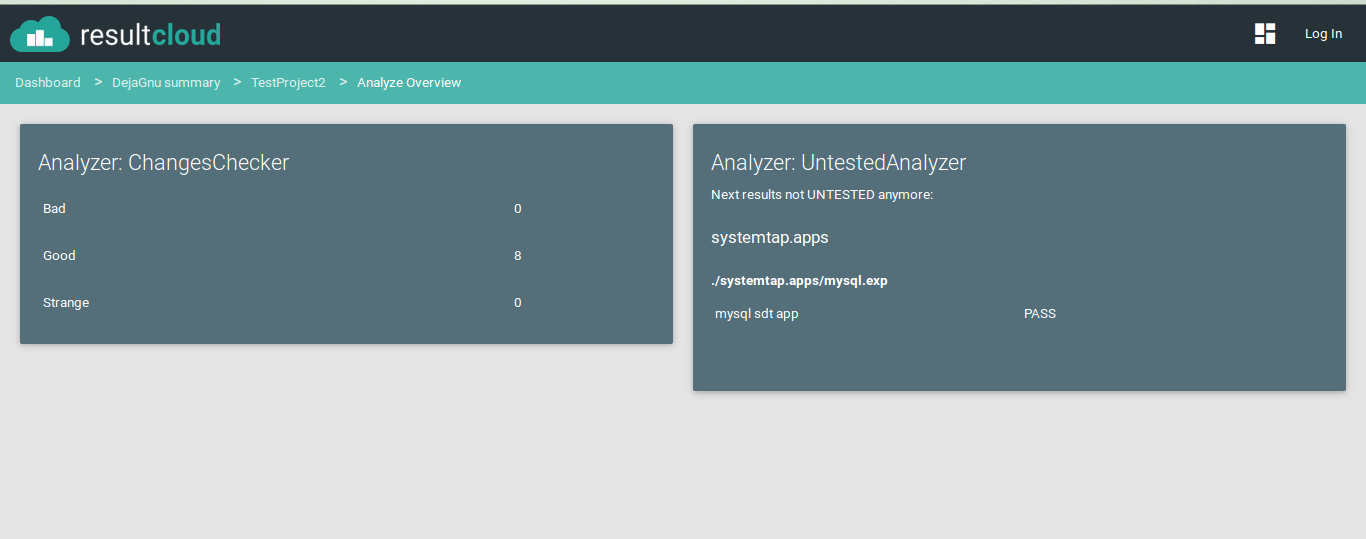
\includegraphics[scale=0.3]{fig/temp_res.png}
  \caption{Implemented template}
  \label{fig:temp_res}
\end{figure}

Analyzer page would use only one component \texttt{analyzeOverview}.It wouldn't have any settings, and will support all plugins. Angular directory first of all get array of analyzing results for current submission, than for each analyzer find own Angular directory, which put analyzer data to template and present it. There some interesting part of code, how is implemented inserting analyzers directive into \texttt{analyzeOverview} component template:
\begin{alltt}
$scope.buildAnalyzerView = function (key) \{
	\textbackslash\textbackslash Check if key not empty
    if (!$(key).length) \{
    	\textbackslash\textbackslash Make new scope clone from rootScope
        var data2 = $rootScope.$new();
        \textbackslash\textbackslash Include into cloned scope analyzer data
        data2.data = $scope.data[key];
        \textbackslash\textbackslash Compile analyzer directive tag with cloned scope
        var el = $compile('<' + key + '/>')(data2);
        \textbackslash\textbackslash Put result into page
        $("#"+key).append(el);
    \}
\}
\end{alltt}

Image\ref{fig:temp_res} presenting how it actually look. 

\texttt{CBuilder} class for \texttt{analyzeOverview} get \texttt{stdClass} object with attribute \emph{Submission} - submission ID. And call \texttt{AnalyzeController} method \emph{VisualizeBySubmission}. \emph{VisualizeBySubmission} get submission ID, for each analyzer get last inserted result, and give it to analyzer's method \emph{VisualizeSingle}, which parse results and return it like array. Then \emph{VisualizeBySubmission} put vizualization data together into associative array the key analyzer ID and value analyze results, and return it.

\chapter{Notification design}

Notification mechanism must be flexible, and easy extended. This chapter contain proposals for implementing notification mechanism.

\section{Architecture}

Like in case with Analyze Controller, I would divide notifications methods to the separated classes and Notification Controller will control them. But as opposed to analyzers there will be several types of notifiers. First type is public notifiers, it means notifications would be send into some shared or public resources, like \emph{Twitter} for example. Private - means it notify each user separetly. According to this private notifiers must have settings, where user can check if he want to get notifications or not, and other options.

\section{Notification Controller}

Notification controller would have method for easy controlling notifications, which get all needed fields, like \emph{title}, \emph{body}, \emph{bodyShort} (for resources that accept only small messages), \emph{adreses} (list of all adreses that must recieve notification) and according to them send notifications. Also \texttt{NotificationController} must provide methods for getting private and public \texttt{Notifiers}. When it will be included, first of all it scan space for available \texttt{Notifiers}.

\section{Notification settings}

There must be mechanism for easy adding settings to \texttt{Notifier}, and settings must be present in user settings without editing any template for it. But user can editing only private settings, because public notifier settings are shared with other users, ResultCloud don't support user hierarchy, thus nobody can edit public notifier settings.

ResultCloud provide good tools for working with settings, like entities \texttt{TemplateSettings} and \texttt{TemplateSettingsItem}. \texttt{TemplateSettings} is for saving into DB setting template information, like setting type, setting name and etc. \texttt{TemplateSettingsItem} is for saving settings value.

\section{Notifier}

\texttt{Notifier} is a base part of notification mechanism, without at least one notifiers it is useless. \texttt{Notifier} provide notification by itself, each notifier has own notification method, for example, by email, or Facebook.

\subsection{Notifiers architecture}

Every \texttt{Notifier} for right work must have unique identifier(ID), by that ID \texttt{NotificationController} would identify notifiers, and in settings template it would have reference to notifier by it ID. \texttt{Notifier} must have one method for notification, and one method with settings. Each notifier has the same settings, thus that method can be pick out into some base paretn class, which would be extended by notifiers classes. \texttt{Notifier} must have attribute that identifies it like private or public notifier.

As a notify method in \texttt{NotificationController}, notify method in \texttt{Notifier} get the same parameters, except address, address will not be associative array, but simple array with addresses supported in that notifier. 

\subsection{Notifier types}

Within the confines of that bachelour work, there must be implemented these types of notifiers:
\begin{itemize} 
\item Email - notifies will be sent by email, this is private notifier
\item Twitter - notifies will be sent into prepared twitter account, public notifier
\item RSS - notifies will be present in RSS file, public notifier
\end{itemize}  

\chapter{Notification mechanism implementation}

This chapter contain description of notification mechanism implementation. As can be seen in image, \texttt{NotificationController} is a kernel, all notifiers are extended from \texttt{BaseNotifier} class.

\section{Structure}

Like analyzers, notification mechanism not a plugin or any else ResultCloud kernel part, thus it also be in \emph{extentions} folder, in own \emph{notification} folder. In root directory is located also \texttt{NotificationController}. All notifiers are located in \emph{notifiers} folder.

Notification start only if analyzer return interesting result.

\section{Settings}

Basically all notifers will have same setting, this settings would enable or disable notification for notifier. But as mentioned in previous chapter, only private notifiers can use settings. Notification mechanism not working with settings, because list of addresses and notifiers must be assamble by those who sending, notification mechanism only get this list and send notification. 

ResultCloud has tools for settings, not only in server side, but also in client side it has automatic form generation for settings. Here is example of default \emph{getSettings} method in \texttt{BaseNotifier} class, for better understanding how set up settings:

\begin{alltt}
public function getSettings()
\{
    \$settings = array();
    \$settingsItem = array();

    \textbackslash\textbackslash Setting label
    \$settingsItem['label'] = "Get notifications by this way";
    \textbackslash\textbackslash Setting ID for TemplateSettings entity
    \$settingsItem['identifier'] = "get-notify";
    \textbackslash\textbackslash Default value
    \$settingsItem['default'] = "1";
    \textbackslash\textbackslash Field type
    \$settingsItem['type'] = TemplateSettingsItemType::CHECKBOX;
    \textbackslash\textbackslash Is setting required
    \$settingsItem['required'] = 'true';
    \$settings[] = $settingsItem;

    return \S$settings; 
\}
\end{alltt}

\section{Notification}

\begin{figure}[hb]
  \centering
    \includegraphics[scale=0.6]{fig/notification_impl.png}
  \caption{Notification mechanism implementation}
  \label{fig:not_impl}
\end{figure}

\subsection{NotificationController}

Like in case with \texttt{AnalyzerController}, \texttt{NotificationController} is static to, all methods are static, because there is no reason to create more than one class instance in application. Notification mechanism scheme\ref{fig:not_impl} showing how \texttt{NotificationController} connecting with other mechanism elements.

When \texttt{NotificationController} is included, first of all start method \emph{preLoad}, that method scan \emph{notifiers} folder, include and assamble array with all available notifiers. For notifing exist function \emph{notify(title, body, bodyShort, to)}, where \texttt{title} - is title of notification message, \texttt{body} - longest body text, \texttt{bodyShort} - short body of the message not longer than 140 letters, \texttt{to} - is an array of all adresses with the key of notifier ID. Function \emph{notify} calling notifier's function \emph{notify}, only for notifiers which have their IDs in \texttt{to} parameter's key.

\texttt{NotificationController} also have different sorts of get methods: \emph{getNotifyIds} (return IDs of all notifiers), \emph{getPrivateNotifiers} (return array with IDs only for private notifiers) and \emph{getNotifierById} (return notifier object by notifier ID).

\subsection{Notifier}

Every notifier must extend \texttt{BaseNotifier} class with default settings, and if needed define own method \emph{getSettings} that in the begining call \emph{parent} method. Also notifier must have unique ID in constant \emph{NOTIFY\_ID}. \emph{NOTIFIER\_PUBLIC} is constant, which contain boolean value, if notifier is public it contain \emph{true}, otherwise \emph{false}. The most important method is \emph{notify}, it has same parameters like method \emph{notify} in \texttt{NotificationController}, except last address parameter, notifier would get not associative array, but simple array with addresses.

\subsection{Notify1}

\texttt{Notify1} is a private notifier that send notifications by email. It get array with email addresses and via default PHP \emph{mail} function send emails. Here notifier parameters:

\begin{alltt}
const NOTIFY_ID = "notify1";
const NOTIFIER_PUBLIC = false;
\end{alltt}

\subsection{Twitter}

\texttt{Twitter} is a public notifier that send new twittes with some interesting information to twitter account. Now it connected to my account \href{https://twitter.com/cyberbond95}{cyberbond95} . If analyzer would have interesting results it send new twitt to my account, and everyone can see it.

\texttt{Twitter} work with Twitter API by using \texttt{TwitterAPIExchange} library, which was suggested in Twitter API documentation. It has MIT license.

\subsection{RSS}

\texttt{RSS} is a public notifier that create or update \emph{rss.xml} file in root folder. \emph{rss.xml} present one news for each project, if \texttt{RSS} get news for already existing in \emph{rss.xml} project, it update news, otherwise it just create new one.

\texttt{RSS} work with RSS by using \texttt{SimpleXML} that is default in mostly PHP versions.

\chapter{Conclusion}

In this bachelor work was proposed mechanism of analyzing tests results and notifing users about it, mechanism must be easy extensible. There must be available more than one notifier for wider using.

Mechanism was built under ResultCloud system by using PHP and JS (AngularJS framework). It consists two part: Analyzers and Notifications. In analyzer part was implemented kernel (\texttt{AnalyzerController}) and one analyzer. In notification part was implemented kernel as well (\texttt{NotificationController}) and three notifiers. And was implemented other parts for integration mechanism into ResultCloud, like services for working with DB, different Angular directives for vizualization data.

%=========================================================================
